\section{Dimensionality Reduction}

\subsection{Motivation}
    \subsubsection{Data Compression}
    Sometimes there exists redundant data dimensions, e.g. repeated quantities in different units. In general, such dimensions are correlated by some hyperbolic surfaces . In the 2D case, two dimensions $x_1, x_2$ can be compressed into a line that describes the correlation of the two dimensions; thus we need only the information of that "line" and where each pair of ($x_1, x_2$) lies on that line (See Figure \ref{fig:data-compression-2-1}). This can further be generalized into more dimensions, e.g. 3 dimensions lying on a 2D-plane (Figure \ref{fig:data-compression-3-2}). 

    We compress the data by projecting the data points on to the plane of correlation approximation and re-coordinate into $z$. This reduces the data to one-less dimension. 
    \begin{figure}[htpb]
        \centering
        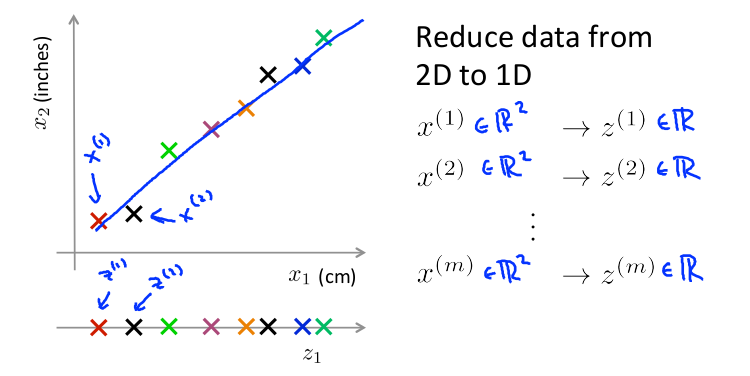
\includegraphics[width=0.8\textwidth]{image/data-compression-2-1.png}
        \caption{Data compression from 2D to 1D}
        \label{fig:data-compression-2-1}
    \end{figure}

    \begin{figure}[htpb]
        \centering
        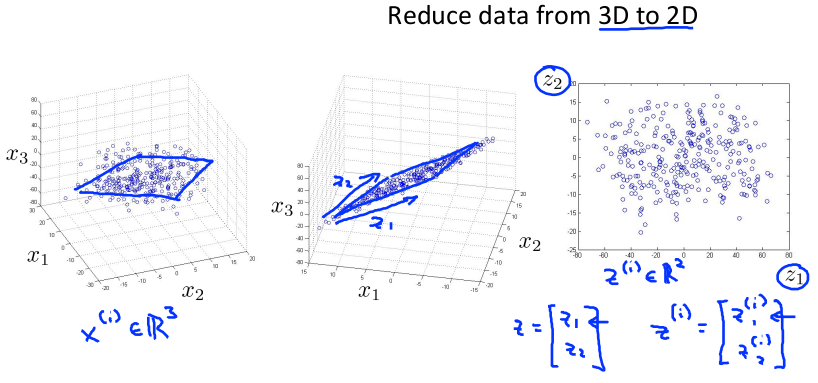
\includegraphics[width=0.8\textwidth]{image/data-compression-3-2.png}
        \caption{Data compression from 3D to 23D}
        \label{fig:data-compression-3-2}
    \end{figure}

    \subsubsection{Data Visualization}
    For visualization purposes, we often wish to group the dimensions into two or three dimensions, of which visualizations are easier perceived by human.

\subsection{Principal Component Analysis}
    \subsubsection{Problem Formulation: n-d to k-d}
    The projection error is the orthogonal distance squared from the data to that projected on the plane.
    To find the plane of correlation approximation, we need to find k vectors: $u^{(1)}, \dots,u^{(k)}$ onto which the data projects, so as to minimize the projection error. We want to project the data onto the linear subspace span by the k vectors. 

    \par For example: from 2D to 1D, we need to find a direction vector ($u^{(1)} \in \mathbb{R}^n$).

    \par Note: \textbf{linear regression is different than PCA.} The former minimizes the squared error $(|y - h(x)|^2)$ (error bar is parallel to the y-axis, not the shortest distance); the latter minimizes the orthogonal distance from the point to the projection. See Figure \ref{fig:linear-regression-PCA} for the comparison.

    \begin{figure}[htpb]
        \centering
        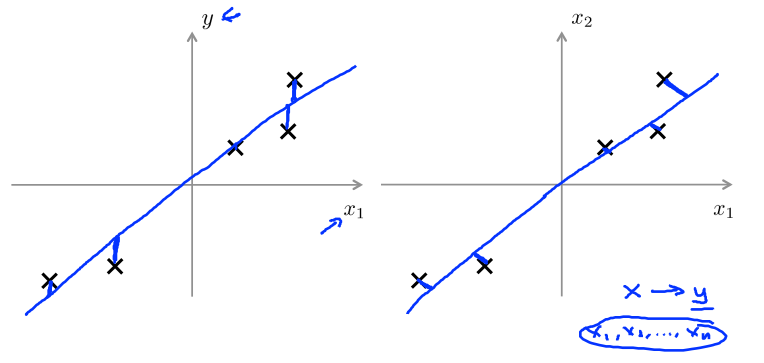
\includegraphics[width=0.8\textwidth]{image/linear-regression-PCA.png}
        \caption{Linear regression vs PCA. Linear regression minimizes the error of y to the prediction. PCA minimizes the error/distance from the original point orthogonal to the projected}
        \label{fig:linear-regression-PCA}
    \end{figure}
\subsection{Principal Component Analysis: Algorithm}
    \subsubsection{Data Preprocessing}
        \begin{itemize}
            \item Training set: $x^{(1)}, x^{(2)}, \dots, x^{(m)}$
            \item Preprocessing (feature scaling and mean normalization):
                \[
                    \mu_j = \frac{1}{m} \sum_{i=1}^{m} x_j^{(i)}
                \] 
                \[
                    x_j^{(i)} \gets \frac{x_j^{(i)} - \mu_j}{s_j}
                \] 
       \end{itemize}

    \subsubsection{Principal Component Analysis}
    Reduce data from n-dimensions to k-dimensions
        \begin{itemize}
            \item Covariance matrix:
                \[
                    \Sigma = \frac{1}{m} \sum_{i=1}^{n} [x^{(i)}][x^{(i)}]^T = \frac{1}{m} X^T X 
                \]

                Recall from Equation \ref{eq:design-matrix}, the design matrix $X$ has each example in a row.

            \item Eigenvectors of $\Sigma$: \verb| [U, S, V] = svd{Sigma}| \\
                  The svd function stands for "single value decomposition". The $U$ matrix is matrix of eigenvectors in columns: 
                  \[
                    U    = \begin{bmatrix}
                    \vertbar    &  \vertbar     &        &     \vertbar \\
                    u^{(1)}     &  u^{(2)}      &  \dots &     u^{(n)}  \\ 
                    \vertbar    &  \vertbar     &        &     \vertbar \\
                           \end{bmatrix}   \in \mathbb{R} ^{n \times n}
                  \] 
              \item Projection: We can take the first k columns from the eigenmatrix U to form $U_{reduce}$:
                  \[
                      U_{reduce}  = \begin{bmatrix}
                        \vertbar    &  \vertbar     &        &     \vertbar \\
                        u^{(1)}     &  u^{(2)}      &  \dots &     u^{(k)}  \\ 
                        \vertbar    &  \vertbar     &        &     \vertbar \\
                                    \end{bmatrix}   \in \mathbb{R} ^{n \times k}
                  \] 
                  Perform the projection:
                  \begin{equation}
                      z^{(i)} = U^T_{reduce} \cdot x^{(i)} \in \mathbb{R}^{k \times 1}
                      \label{eq:pca-projection}
                  \end{equation} 
        \end{itemize}

\subsection{Reconstruction from compressed representation}
    We can guess the original data by inverting \ref{eq:pca-projection}.
    \[
        x \approx x_{approx} = U_{reduce} \cdot z
    \] 

\subsection{Choosing k (num of principal components)}

    \begin{itemize}
        \item Average squared projection error: $\frac{1}{m} \sum_{i=1}^{n} \| x^{(i)} - x_{approx}^{(i)} \| ^2$
        \item Total variation in data: $\frac{1}{m} \sum_{i=1}^{n} \| x^{(i)} \|^2$
        \item Choose k s.t. "99\% variance is retained":
            
            \begin{equation}
                \frac{ \frac{1}{m} \sum_{i=1}^{n} \| x^{(i)} - x_{approx}^{(i)} \| ^2}{\frac{1}{m} \sum_{i=1}^{n} \| x^{(i)} \|^2} \leq  0.01
                \label{eq:pac-metric}
            \end{equation} 
            
        \item Procedure: Try PCA with k=1, compute $U_{reduce}$, check Equation \ref{eq:pac-metric}, $k\gets k+1$.
        \item Implementation note: Equation \ref{eq:pac-metric} can be solved differently using the $S$ matrix. $S \in \mathbb{R} ^{n \times n}$ is a diagonal matrix. For a given k, we can compute Equation \ref{eq:pac-metric} by: 
            \[
                1 - \frac{\sum_{i=1}^{k} S_{ii}}{\sum_{i=1}^{n} S_{ii}}
            \], or alternatively,  
            \[
                \frac{\sum_{i=1}^{k} S_{ii}}{\sum_{i=1}^{n} S_{ii}} \geq 0.99
            \] 

    \end{itemize}
\subsection{Advice for applying PCA}
    \begin{enumerate}
        \item Supervised learning speed-up: define the mapping $x^{(i)} to z^{(i)}$ by running PCA on the \textbf{training set}. This mapping can be later used on cross validation and test sets.
        \item Application of PCA
            \begin{enumerate}
                \item Compression (reduce space), speed up learning algorithm.
                \item Visualization.
                \item \textbf{Bad usage}: prevent overfitting (fewer features, less likely to overfit). However, PCA discards certain information through the projection step. It is better to use regularization ($\lambda$)
            \end{enumerate}
        \item Design ML system without PCA first, if that doesn't work, then try PCA.
    \end{enumerate}
